\subsection{Armazenamento}

	Neste projeto será utilizada a câmera VIP E5120 IR. É uma câmera já voltada para sistemas de vigilância, muito utilizada em escritórios e shoppings.

	\begin{table}[H]
		\centering
		\begin{tabular}{|l|l|}
			\hline
			Resolução           & 1280/960       \\ \hline
			Quantidade de MP    & 1.3 MegaPixels \\ \hline
			Sensor              & Infravermelho  \\ \hline
			Alimentação         & 24Vac a 3$^a$  \\ \hline
			Compressão de vídeo & H264/MJPEG     \\ \hline
		\end{tabular}
		\caption{Especificações da VIP E5120 IR fonte: \cite{mercadoLivreVIPE5120}}
		\label{my-label}
	\end{table}

	Serão utilizadas, no total, 15 câmeras do modelo VIP E5120 IR, e para manter um armazenamento dessa quantidade vídeo, seria necessário um HD realmente potente e para tanto será utilizado o Seagate® Vídeo 3.5 HDD. Como o sistema funcionará  24x7, ou seja, 24 horas por 7 dias da semana, o servidor irá passar as imagens para o HD a uma taxa de 768 Kbps, em um mês (considerando um mês como 30 dias), será gasto um total de 3.5TB.

\begin{table}[H]
	\centering
	\begin{tabular}{|l|l|}
		\hline
		Capacidade                  & 4TB            \\ \hline
		Modelo                      & ST400DM000     \\ \hline
		Interface                   & SATA de 6 GB/s \\ \hline
		Velocidade da rotação       & 5900 RPM       \\ \hline
		Cache                       & 64 MB          \\ \hline
		Impacto máximo de operação  & 80 Gs          \\ \hline
		Tipo de armazenamento       & HDD            \\ \hline
		Comprimento                 & 147.00 mm      \\ \hline
		Largura                     & 101.85 mm      \\ \hline
		Altura                      & 26.1 mm        \\ \hline
		Peso típico                 & 610 g          \\ \hline
		AFR                         & 0.55\%         \\ \hline
		Potência média de operação  & 7.500 W        \\ \hline
		Taxa de transferência       & 600 MB/s       \\ \hline
		Taxa de dados sustentada DE & 180            \\ \hline
	\end{tabular}
	\caption{Especificações da Seagate$^{\textregistered}$ Vídeo 3.5 HDD \cite{seagate}}
	\label{my-label}
\end{table}

\begin{table}[H]
\centering
\begin{tabular}{|l|l|}
\hline
Processador              & Intel Core i7 - 4700K                                                   \\ \hline
Placa-mãe                & ASRock Z87Killer                                                        \\ \hline
Memoria                  & 16 GB G. Skill Spiner (DDR 3 - 1600/PC3 - 12800), configurada a 1600MHz \\ \hline
Placa de vídeo           & GeForce GT 630 1GB                                                      \\ \hline
Resolução de vídeo       & 1920x1080                                                               \\ \hline
Fonte de alimentação     & Corsair CX500M                                                          \\ \hline
Unidade de inicialização & Kingston HyperX 3k 480 GB                                               \\ \hline
\end{tabular}
\caption{Configuração de Hardware}
\label{tab:configHardware}
\end{table}

As câmeras serão fixadas ao balão, quando acondicionadas em seus respectivos invólucros
ou caixas de proteção. Deverão continuar operando perfeitamente sob temperatura ambiente
entre 0 e 40$^{\circ}$C e umidade relativa do ar de até 90\%.

Em tempos de muitas chuvas, ocorre uma grande variação de energia, devido às descargas
elétricas de raios. Para que não se tenha o problema de o sistema parar de funcionar por falta de
energia, e pela variação de energia, não chegar a queimar o sistema ou danificar o sistema,
será utilizado um equipamento que armazenar energia por algum tempo.

O equipamento utilizado para o sistema de energia nobreak, será o \textbf{Nobreak Organizador e
Fonte para 16 câmeras}, da tecnologia ONAT. Com este equipamento, o armazenamento de
dados terá em média 4 horas de autonomia, ou seja, caso por algum motivo a luz acabe o
sistema terá em média 4 horas funcionando perfeitamente \cite{nobreak}.

O Seagate para gravação e backup de imagens deverá ser alimentado pelo sistema de energia
(nobreak), de forma a possibilitar a operação em caso de falta de energia elétrica.

\begin{table}[H]
\centering
\begin{tabular}{|l|l|l|l|}
\hline
                      & Unidades & Preço de uma unidade & Preço total    \\ \hline
Câmera VIP E5120 IR   & 15       & R\$ 8.728,10         & R\$ 130.921,50 \\ \hline
Seagate$^{\textregistered}$ Vídeo 3.5 HDD & 4        & R\$ 984,90           & R\$ 3.939,60   \\ \hline
Sistema Nobreak       & 1        & R\$ 396,90           & R\$396,90      \\ \hline
Hardware              & 1        & R\$ 5.271,86         & R\$5.271,86    \\ \hline
\multicolumn{4}{|r|}{R\$ 140.529,86}                                     \\ \hline
\end{tabular}
\caption{Tabela de preços}
\label{table:precosComponentes}
\end{table}

\subsection{Sistema de comunicação Estação solo - Vigilante segurança}

O sistema de comunicação será dado de maneira manual, ou seja, terá uma pessoa na estação
de solo que será responsável por analisar os monitores de vigilância que  informam as áreas de possíveis situações de risco mediante a pontuação preestabelecida no sistema. E caso seja necessário, o operador irá alertar um segurança para que ele possa averiguar tal situação. O sistema será uma ferramenta para o operador, auxiliando e facilitando o monitoramento do estacionamento.

Essa comunicação será dada via voz, utilizando um rádio comunicador, ou walk talk. Este meio
de comunicação é bem utilizado em sistemas de vigilância de escritórios, shoppings, em
 construções civis ou em operações de policiais e bombeiros.

Os Walkie Talkies tem um alcance relativamente alto, exatamente o necessário para suprir a
carência de sinal de celular presente na área da FGA, e este equipamento terá um alcance de
 56km. Neste sistema de monitoramento será utilizado o rádio comunicador walk talk Cobra
Cxr925 56km.

\begin{table}[H]
\centering
\begin{tabular}{|l|l|}
\hline
Peso        & 68g                          \\ \hline
Alcance     & 56 km                        \\ \hline
Dimensões   & 177,50mm x 49,00mm x 33,00mm \\ \hline
Frequência  & 22 canais                    \\ \hline
Alimentação & 110 V                        \\ \hline
Preço       & R\$ 415,99                   \\ \hline
\end{tabular}
\caption{Especificações e preço do Walk Talk Cobra Cxr925 56km \cite{walk}.}
\label{table:walk}
\end{table}

\subsection{Processamento dos dados}

Para o armazenamento se tornar eficiente e confiável, além de resiliente, será implementado o
padrão RAID(\textbf{Redundant Array of Independent Disks}) em seu nível um também conhecido por
Mirror.

Todas as informações vindas processadas para armazenamento serão copiadas
simultaneamente em dois HDs, reduzindo a performance porém mantendo assim a segurança,
pois caso haja algum problema técnico em um dos armazenamentos, não haverá nenhuma
perda de informação. Neste projeto serão utilizados 4 Seagate® Vídeo 3.5 HDD para o
armazenamento das imagens do monitoramento, formando 2 pares de HDs, que serão
redundantes \cite{raid}.

Cada par será capaz de armazenar informações por 30 dias, uma vez cheio as informações passarão a ser armazenadas no par ocioso, formando assim um total de 60 dias de armazenamento de informação, ao final deste período, informações armazenadas serão a ser eliminadas, sendo assim necessário realizar cópias para outros dispositivos caso seja necessário o uso em um período posterior.O tempo em média para recuperação das imagens será de uma a duas horas.

\subsubsection{Redundância de software}

Um software bem projetado corretamente desde a sua elaboração, não necessita de técnicas de tolerância para software, mesmo que ainda não seja possível garantir na pratica que todo programa estarão corretos \cite{webertolerancia}.

As formas usuais de redundância de software são:

\begin{itemize}
	\item Diversidade (ou programação n-versões)
	\item Blocos de recuperação
\end{itemize}

\paragraph{Diversidade}

Diversidade, também chamada programação diversitária, é uma técnica de redundância usada para obter tolerância a falhas em software. A partir de um problema a ser solucionado são implementadas diversas soluções alternativas, sendo a resposta do sistema determinada por votação.

Os erros,para poderem ser detectados, devem se manisfestar de forma diferente nas diversas alternativas, ou seja, devem ser estatisticamente independentes. Experimentalmente foi comprovado que o numero de erros idênticos(erros que não seriam detectados) é consideravelmente menor que o numero total de erros.

Diversidade pode ser utilizada em todas as fases de desenvolvimento do projeto. Essa técnica é chamada de projeto diversitário quando o desenvolvimento do sistema é ralizado de forma diversitároa e de programação em varias versões quando se restringe á implementação do sistema.

Os pontos negativos dessa técnica devem ser colocadas em pauta, como o aumento dos custos de desenvolvimento e manutenção, a complexidade de sincronização das veres e o problema de determinar a correlação das fontes de erro.

\paragraph{Blocos de recuperação}

Nessa técnica programas secundários só serão necessários na detecção de um erro no programa primário.Essa estratégia envolve um teste de aceitação.Programas são executados e testados um a um até que o primeiro passa no teste de aceitação. A estratégia de blocos de recuperação tolera n-1 falhas, no caso de falhas independentes nas n versões.



\begin{figure}[H]
		\centering
		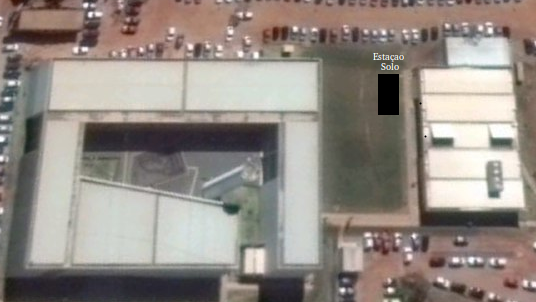
\includegraphics[width=0.6\textwidth]{figuras/estacaoSolo}
		\caption{Local da Estação Solo}
		\label{img:estacaoSoloLocal}
	\end{figure}
